
\chapter{Stretching our legs}
\label{ch:intro}

We've got a steep climb up ahead of us. What exactly are we up against? And
what will we see from the summit that will be worth all the effort to get
there?

As we did in the opening chapter of \textit{A Cool, Brisk Walk}, let's take the
two words of our subject -- ``Linear Algebra'' -- one at a time, and talk about
what they mean. And just like we did for ``Discrete Mathematics,'' we'll
consider the words in reverse order.

\section{``Algebra''}

\index{Algebra}
When most people hear the word ``algebra,'' they flash back to middle school,
to that subject where they first learned to work with letters (like $x$)
instead of just numbers (like 5) in a math class. They remember the quadratic
formula, collecting like terms, factoring expressions, and so on.

\index{algebra@``an algebra''}
That middle school class is indeed related to the subject of our book, but more
distantly than you might imagine. Properly speaking, that middle school subject
is a \textit{proper} noun: ``Algebra'' with a capital `A.' It's actually a
special case of the \textit{common} noun that mathematicians deal with: an
``algebra'' with a lower-case `a.' Okay. So what's ``\textit{an} algebra,''
then?

\index{object, mathematical}
\index{mathematical object}
\label{mathematicalObject}
An algebra is any system of mathematical objects together with operations that
can be used to combine them. The middle school Algebra is an example: the
``objects'' are numbers (or letters that stand for numbers) and the operations
are things like addition, multiplication, powers, roots, and the like. We can
take numbers (or stand-ins) like:

\vspace{-.25in}
\begin{align*}
5, x, 3, y, q, 17, 14, z, 9
\end{align*}

and combine them to build up a complex expression like:

\vspace{-.25in}
\begin{align*}
\frac{\frac{(5+x)^3}{y} - q\cdot 17}{\sqrt{(14+x)^z + 9+y}}.
\end{align*}

It looks kinda gross, but I think you'll agree that if you knew what numbers
each letter stood for, you could laboriously crank out the answer with a
calculator.

Another example was the algebra of sets we learned about in \textit{Cool, Brisk
Walk} chapter 2. We could take the sets $A, B, \mathbb{N},$ and $\mathbb{Q}$
and combine them with set operations to get:

\vspace{-.25in}
\begin{align*}
((A \cap \mathbb{N}) \cup \overline{B}) \times A - \overline{(\mathbb{Q} \cup
B)}.
\end{align*}

Or, from chapter 8 of \textit{Cool, Brisk Walk}, we could combine the logical
propositions $P, Q, R,$ and $S$ to get a compound proposition like:

\vspace{-.25in}
\begin{align*}
(\neg P \vee Q \wedge \neg (R \oplus P)) \Leftrightarrow (\neg S \Rightarrow P).
\end{align*}

Any system of mathematical objects and operations like this is an ``algebra.''
The subject of this book is \textit{linear} algebra in which the ``mathematical
objects,'' instead of being numbers or sets or propositions, are
\textbf{vectors} and \textbf{matrices}.

\subsection{Closure}
\index{closure}

Key to the notion of an algebra, by the way, is the notion of \textbf{closure}.
Closure means that when we combine two or more of the mathematical objects in
question, we get back another object \textit{of the same type.} For instance,
whether or not you can simplify $\frac{227}{45}$ in your head, you \textit{do}
know that when you divide 227 by 45 you will get \textit{a number}. Similarly,
if you take the union of two sets $D \cup M$, you will get \textit{a set}. And
if you take the exclusive-or of two propositions $L \oplus A$, you will get
\textit{a proposition}.

\index{porcupine}

This is important because without this guarantee, we couldn't build up complex
expressions and be certain they would mean anything. Take the expression $12 +
\frac{227}{45}$. Even without a calculator, you know these operations can in
principle be done, because whatever exact value $\frac{227}{45}$ turns out to
be, it's guaranteed to be \textit{a number}, and therefore it can be
meaningfully added to 12. If, when dividing one number by another, the result
might wind up being a \textit{set} (or a proposition, or a porcupine), then the
whole expression would become meaningless: you can't add a number to a
porcupine.

In this book we'll combine vectors and matrices in a myriad of different ways,
and we will always get vectors and matrices back. That's why they constitute
``an algebra.''

\section{``Linear''}

\index{linear}
\index{function}

The word \textit{linear} is related to the word \textit{line}: this is because
a function that is linear looks like a line when it's plotted.\footnote{Now
there's one confusing detail I want to clear up right away. You'll recall that
in high school, you learned that the equation for a straight line was
\index{y=mx+b@$y=mx+b$} ``$y=mx+b$''. Would it surprise you if I told you that
this is \textit{not} considered a linear function, according to the worldview
of this book? Yep.~:\textbackslash~Sorry for the surprise. That high school
thing is actually called an \index{affine function} \textbf{affine} function
rather than a linear function. The reason is the $b$, also called the
\index{y-intercept@$y$-intercept} $y$-intercept. If $b$ is anything other than
zero, then neither of the two ``linear expectations'' that we'll see on
p.~\pageref{linearExpectations} will be true. For example, if $f(x)=3x+7$, then
$f(2)$ (which is 13) won't be $2\cdot f(1)$ (which is 20), as our linearity
definition requires. For us in this book, the only functions considered
``linear'' are those lines that \index{origin} \textit{pass through the
origin}, and thus have a $y$-intercept of 0.} Suppose I make \$11.75/hour at my
part-time job, and I want to figure out my take-home pay for last week's work.
Obviously, my paycheck (before taxes and what-not) will be 11.75 times the
number of hours I work. The left side of Figure~\ref{fig:linearNLPlots} shows
my hours vs.~my pay, which is, not surprisingly, a line.

\begin{figure}[ht]
\centering
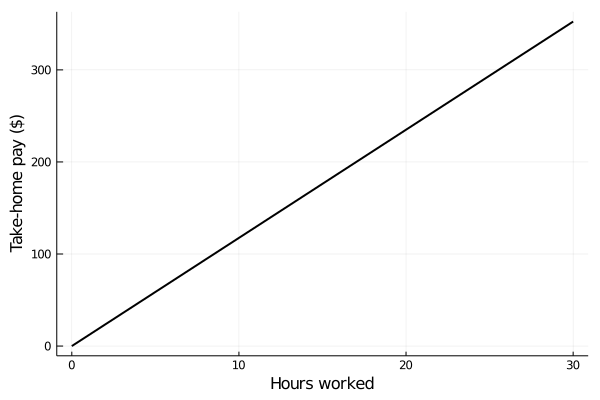
\includegraphics[width=0.45\textwidth]{linear.png}
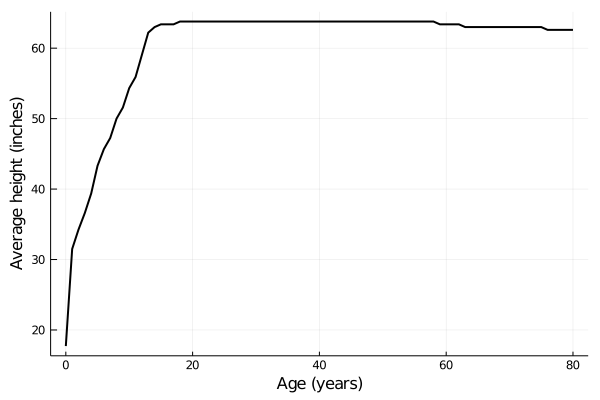
\includegraphics[width=0.45\textwidth]{nonlinear.png}
\caption{Linear and non-linear functions.}
\label{fig:linearNLPlots}
\end{figure}

By contrast, suppose I wanted to predict how tall a typical American human
female would be based on her age. While it's true that for most age ranges the
two variables increase together (just as more hours-worked implies more
take-home pay, so does more years-on-earth implies more inches-off-the-ground),
the plot is no longer a straight line (see the right side of
Figure~\ref{fig:linearNLPlots}).

It's worth lingering for a moment on what linear \textit{means} and how it
colors our assumptions about what to expect. Imagine this conversation:

\begin{dialogue}

\speak{You} Hey boss, I know I'm normally only scheduled to work for 12 hours a
week, and I get 120 bucks for that. But I need to start saving up for a plane
ticket to see my grandparents, so I'd like to work 15 hours next week. That
okay?

\speak{Boss} Sure, you can do 15 next week. That'll make your take-home
pay an even \$5,000 for the week.

\speak{You} \direct{Jaw drops open} Whoa, five \textit{grand}?! Heck, in that
case, push me up to 20 -- I can make some headway on my fall tuition!

\speak{Boss} Twenty hours it is -- you'll earn a total of 75\textcent~for
that.

\speak{You} \textit{D'oh!!}

\end{dialogue}

The above dialogue is absurd. But exactly \textit{why} is it absurd? Answer:
because we expect weekly-pay-vs.-hours-worked to be linear, and the values
given in the dialogue violate our linear assumptions.

\bigskip
The following scene, by contrast, \textit{isn't} absurd:

\begin{dialogue}

\speak{You} It's now been 12 months since I bought it, and my Blackberry stock
is currently worth \$120. Dear Crystal Ball, how much will it be worth three
months from now (at the 15-month point)?

\speak{Crystal Ball} Blackberry will skyrocket in the public's imagination
three months from now, so at the 15-month mark your stock will be valued at
\$5,000.

\speak{You} Woo-hoo! And how about at the 20-month mark?

\speak{Crystal Ball} Unfortunately for shareholders, Blackberry Inc.~will make
some bad business decisions and crash. The stock will be nearly worthless --
just 75\textcent.

\speak{You} Yikes -- glad I asked! Please sell it in three months, okay?

\end{dialogue}

This scenario doesn't seem out of the question because we have no expectations
about stock prices being linear in time.

\medskip

\index{expectations, linear}
\index{linear expectations}
So what exactly are those linear expectations? If you work it out, they come
down to two:

\definecolor{shadecolor}{rgb}{.9,.9,.9}
\begin{framed}
\label{linearExpectations}
If a function $f(x)$ is linear, then:
\begin{compactitem}
\item $f(a\cdot x)$ is always simply $a\cdot f(x)$.
\item $f(x+y)$ is always simply $f(x)+f(y)$.
\end{compactitem}
\end{framed}

Take the first one. Let's say Wawa is selling a King Size Kit Kat bar for
\$1.50. How much would four bars cost? The answer's got to be \$6.00. It would
be weird to be anything else. In this example, $x$ is the number of Kit Kat
bars, and $f(x)$ is the total cost. $f(x) = 1.5x$, and predictably, $f(4\cdot
1) = 4 \cdot f(1) = 4 \cdot 1.5 = 6.$

For the second rule, let's say we bought two Kit Kat bars today and three more
tomorrow. How much for the total? If the universe is working normally, buying
two today and three tomorrow would be the same price as buying five altogether.
And it's true: $f(2+3) = f(2) + f(3) = 3 + 4.5 = 7.5 = f(5)$. It would be weird
to work any other way.

When we have non-linear functions, we don't expect these things to be true. If
my nine-year old daughter is 4 feet tall, I don't expect her to be 8 feet tall
when she turns eighteen. $f(a\cdot x) \neq a\cdot f(x)$. And if my Blackberry
stock is worth \$5,000 after sixteen months and \$100 after the company's
disastrous seventeenth, we don't count on it being worth \$5,100 after 33
months. $f(x+y) \neq f(x)+f(y)$.

For the rest of this entire book, the two assumptions above will always be
true. It may seem limiting, but as we've seen, there are lots of cases where it
simply doesn't make any sense for our function \textit{not} to be linear.

\section{This book contains only elephants}

\index{elephants}
\index{Ulam, Stanis\l{}aw}

The great mathematician and computational scientist Stanis\l{}aw Ulam once
quipped that dividing functions into linear and non-linear is like dividing
zoology into ``elephant'' and ``non-elephant.'' In a way it's true, because
there are certainly far more functions that \textit{don't} obey the above two
properties than there are those that do. By the same token, though, there are
far more pay schemes we could invent than just ``a regular hourly rate.'' But
hourly rates come up very, very often, and when they do, there's a lot of
amazingly useful things we can do with them. Join us on our hike and you'll
see.

\bigskip
\hrulefill \\

\pagebreak

\section*{\faPython \ \ \textit{Appendix: Python}}

\index{Python}
\index{programming}
\index{calculator, glorified}

Each chapter of this book comes equipped with an appendix showing how to carry
out the various linear algebra calculations in a programming language called
Python. Here's the first one!

\medskip

Most readers will have done at least a little bit of computer programming
before making it to this book. If you haven't, don't worry about it. We're not
really going to be programming \textit{per se}, but rather using the Python
language as a glorified calculator.

Python is of course a fully-functional, feature-rich programming language that
can be used for just about any program you want to write, whether that's a PC
or smartphone app, a data analysis program, or a dynamic website. It's a great
and very readable language, and I highly recommend adding it to your quiver as
you assimilate various high-tech tools.

\subsection*{Installing and navigating Python}
\index{NumPy}
\index{Anaconda}
\index{Spyder}
\index{code}
\index{debug}
\index{console window}
\index{editor window}

For this book, all you'll need to do is download a Python IDE\footnote{IDE
stands for ``Integrated Development Environment'' and just means ``a
point-and-click interface that lets you write programs, edit them, run them,
and debug (find and remove errors) them.''} and the ``package'' (bundle of
software) called ``\textbf{numpy}.'' NumPy\footnote{NumPy can be pronounced
either ``NUM-PIE'' or ``NUM-pee.'' I've heard both.} stands for ``numerical
Python,'' and has the various cogs and gears to create vectors and matrices,
the mainstays of this book. The easiest way I know of to do this is to download
the \textbf{Anaconda} Python distribution from \url{www.anaconda.com}, and then
start the \textbf{Spyder} application that automatically comes with it.

Whether you use Spyder or a different IDE (IDLE, Eclipse, and PyCharm are some
other popular ones), the main thing to focus on -- and the only thing I'll
describe in this book -- is the Python code itself, which you'll type in an
\textbf{editor} window that sorta resembles Microsoft Word or Google Docs.

After you type in some code and want to try running it, you'll execute whatever
the ``run/execute'' operation is in your IDE (in Spyder it's a little green
``run'' arrow). The output of the code will then appear in some kind of
\textbf{console} window (normally another pane on the screen; in Spyder it's on
the lower-right by default). Just think of this like a calculator: you first
type in something like ``\texttt{258 $\times$ 312}'' and then when you press
the equals sign (\texttt{=}) the answer \texttt{80496} appears.

That's more or less all we'll be doing in this book. The code you write in the
editor window will be like the ``\texttt{258 $\times$ 312}'' part (except it
will involve vectors and matrices), and the \texttt{80496} is what Python will
print to the console window. Our ``programs'' won't even really deserve the
name.

From now on, whenever I give example Python code in this book, I'll write it in
a box like this:

% TODO: update year from 2021 to whatever. (See several places below where
% values are referenced.)

\label{firstPython}

\vspace{-.15in}
\begin{Verbatim}[fontsize=\small,samepage=true,frame=single,framesep=3mm]
# Our first code example!
from numpy import *

founding = 1776
usa_age = 2021 - founding
print("Our country is {} years old!".format(usa_age))
\end{Verbatim}
\vspace{-.15in}

That box means ``this stuff goes in the editor window.''

\medskip

When I write the corresponding output (\textit{i.e.}, what gets printed to the
console when you run the code) I'll write it like this:

\vspace{-.1in}
\begin{Verbatim}[fontsize=\small,samepage=true,frame=leftline,framesep=5mm,framerule=1mm]
Our country is 245 years old!
\end{Verbatim}
\vspace{-.1in}

That vertical bar means ``this stuff is the printed result of executing that
code.''

\medskip

\subsection*{First steps}

And actually, before we end this first appendix, let's talk briefly about the
code in that very first box and what it means.

\index{hashtag}
\index{commenting out code}

First off, you'll see that the first line of that code snippet begins with a
hashtag (``\texttt{\#}''). This tells Python to \textit{ignore} that line
entirely. It doesn't contain Python code, after all, but English text, which
Python can't understand. This is called a \textbf{comment}. Comments are used
quite often as ``notes to oneself,'' to organize a program, or to narrate
non-obvious sections of code.

Another use of the hashtag (perhaps even more common) is to temporarily
``comment out'' lines of code that you don't want to run for the time being.
Instead of outright deleting things you want Python to ignore for the moment,
it's convenient to stick hashtags on the far-left of such lines, since you can
easily remove the hashtags whenever you want to get Python to recognize those
lines again.

\smallskip

Moving on, the very first (non-commented) line of code you'll put in every
Python program is this one:

\begin{Verbatim}[fontsize=\small,samepage=true,frame=single,framesep=3mm]
from numpy import *
\end{Verbatim}

which just means ``I'd like to use the NumPy package, please.''\footnote{You
may see other ways of importing NumPy, particularly this one:

\medskip
\quad\quad\texttt{import numpy as np}
\medskip

This is actually slightly better practice, but it also means that any time
you'd want to use NumPy stuff -- like the \texttt{array()} function we'll talk
about in Chapter~\ref{ch:vectors} -- you'd have to prefix it with
``\texttt{np.}'' It's slightly more convenient to avoid that for our
Python-as-quick-calculator approach.}

\smallskip

\index{variable (Python)}
\index{assignment (Python)}

The next two lines of code create \textbf{variable}s, which are named
containers that hold values. In this case, the values in question are simply
integers, although later in the book we'll be using variables to store vectors
and matrices and other goodies.

To create a new variable (or change the current value of an existing variable),
you simply give the variable a name (with no spaces or funky characters) and
use the equals sign to \textbf{assign} that variable a value, as in
``\texttt{founding = 1776}''. Unlike in math, a program variable's value can
change throughout the program any time the code assigns it a new value.

The following line is only slightly more complicated: it performs a subtraction
operation to \textbf{calculate} a value for the \texttt{usa\_age}
variable.\footnote{Underscores are commonly used in variable names to split up
multiple words. Underscores are \textit{not} considered ``funky.''} Some of the
symbols used for common mathematical operations are obvious, and some are not:

\begin{compactitem}
\item[\texttt{\large +}]-- addition
\item[\texttt{\large -}]-- subtraction
\item[\texttt{\large *}]-- multiplication
\item[\texttt{\large /}]-- division
\item[\texttt{\large \%}]-- modulus (``remainder when dividing by'')
\item[\texttt{\large **}]-- exponentiation (``to the power of'')
\end{compactitem}

\medskip

Finally, the last line (with \texttt{print()}) is used for displaying output to
the console. Inside the parentheses, you put a quoted piece of text that you
want to display. You put a pair of back-to-back curly braces
(``\texttt{\{\}}'') to create a placeholder for a variable's value to be
inserted. Then, following the final quotation mark, you put
``\texttt{.format()}'' (notice the leading dot) and inside \textit{its} parens
you list the variables (separated by commas if they're more than one) that you
want Python to substitute in the placeholders. Make sure you get the syntax
right, character-for-character, because like most programming things it's
error-prone and unforgiving.

\medskip

Code in a Python program executes line-by-line, top-to-bottom. So after the
NumPy library is imported, and the \texttt{founding} variable is given the
value 1776, the next line subtracts 1776 from 2021 and sets \texttt{usa\_age}
to 245. The print statement then sticks that value in for the placeholder in
its message, and outputs the complete message to the screen: ``\texttt{Our
country is 245 years old!}''

\bigskip

That's it! After you've typed this example program into Spyder's (or your
IDE's) editor, and run it to see the output shown above in the console, I
hereby declare you Python-ready for the rest of the book.
